\documentclass[mathserif,hyperref]{beamer}

\usepackage[spanish]{babel}
\usepackage[utf8]{inputenc}
\usepackage{amsmath}
\usepackage{array}
\usepackage{caption}
\usepackage{adjustbox}
\usepackage{lmodern}

\usetheme{Luebeck}
\usecolortheme[rgb={0.67,0.05,0}]{structure}
\usecolortheme{beaver}

% elimina las siguientes advertencias:
% LaTeX Font Warning: Font shape `OT1/cmss/m/n' in size <4> not available
% (Font)              size <5> substituted on input line 22.
% LaTeX Font Warning: Size substitutions with differences
% (Font)              up to 1.0pt have occurred.

\title{Prueba de oposición}
\author{Lucas Gabriel Vuotto}
\date{\today}


% Adicional intercala package{beamerthemeshadow}
%\usepackage{beamerthemeshadow}
%  causa que elementos que aparece en el futuro
%  escribe ligero
%\beamersetuncovermixins{\opaqueness<1>{25}}{\opaqueness<2->{15}}
% funciona por tablas tamb\'\i en cuando aplica teTeX$B!D(B
\begin{document}


\section{Ejercicio}

\begin{frame}
\frametitle{Enunciado}
\textbf{Ejercicio 11}
{\tiny Organización del Computador I - práctica 2 (lógica digital) - segundo
cuatrimestre del 2014.}
\begin{enumerate}
  \item Diseñar un \textit{sumador completo} de 1 bit usando sólo compuertas
  NAND.
  \item Suponiendo que todas las compuertas elementales tienen el mismo
  retardo \textit{(delay)} $t$, calcule el retardo total del circuito para
  producir todas sus señales de salida.
\end{enumerate}
\end{frame}


\begin{frame}
\frametitle{\small Diseñar un \textit{sumador completo} de 1 bit usando sólo
compuertas NAND}
Tablas de verdad
\begin{columns}
  \column{.5\textwidth}
    \begin{center}\begin{table}
    \begin{tabular}{| c | c || c | c |}
      \hline
      $e_0$ & $e_1$ & $c$ & $s$ \\ \hline
        0   &   0   &  0  &  0  \\
        0   &   1   &  0  &  1  \\
        1   &   0   &  0  &  1  \\
        1   &   1   &  1  &  0  \\
      \hline
    \end{tabular}
    \caption*{Sumador simple}
    \end{table}\end{center}
  \column{.5\textwidth}
    \begin{center}\begin{table}
    \begin{tabular}{| c | c | c || c | c |}
      \hline
      $e_0$ & $e_1$ & $c_e$ & $c_s$ & $s$ \\ \hline
        0   &   0   &   0   &   0   &  0  \\
        0   &   1   &   0   &   0   &  1  \\
        1   &   0   &   0   &   0   &  1  \\
        1   &   1   &   0   &   1   &  0  \\
        0   &   0   &   1   &   0   &  1  \\
        0   &   1   &   1   &   1   &  0  \\
        1   &   0   &   1   &   1   &  0  \\
        1   &   1   &   1   &   1   &  1  \\
      \hline
    \end{tabular}
    \caption*{Sumador completo}
    \end{table}\end{center}
\end{columns}
\end{frame}


\begin{frame}
\frametitle{\small Diseñar un \textit{sumador completo} de 1 bit usando sólo
compuertas NAND}
\begin{figure}[htp]
  \caption{Sumador simple}
  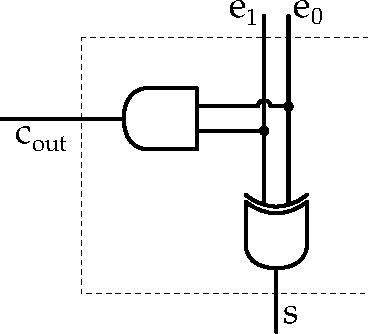
\includegraphics[scale=0.9]{sumador-simple.pdf}
\end{figure}
\end{frame}


\begin{frame}
\frametitle{\small Diseñar un \textit{sumador completo} de 1 bit usando sólo
compuertas NAND}
\begin{figure}[htp]
  \caption{Sumador completo}
  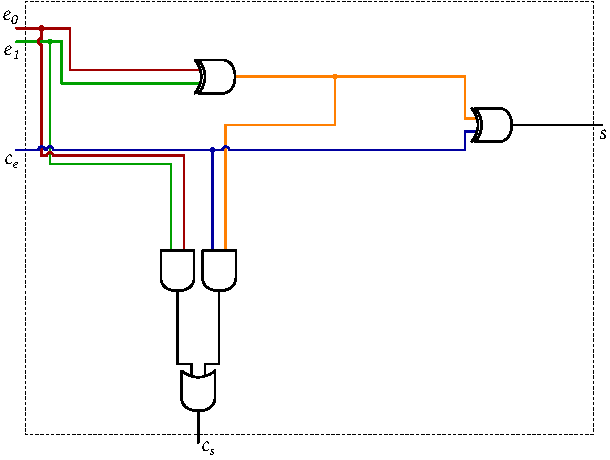
\includegraphics[scale=0.7]{sumador-completo.pdf}
\end{figure}
\end{frame}


\begin{frame}
\frametitle{\small Diseñar un \textit{sumador completo} de 1 bit usando sólo
compuertas NAND}
\begin{center}Método matemático\end{center}
\begin{align*}
  s   &= e_0 \oplus e_1 \oplus c_e \\
  c_s &= (e_0 . e_1) + (e_0 \oplus e_1) . c_e
\end{align*}
\begin{center}{\Large ¡Aburrido!}\end{center}
\end{frame}


\begin{frame}
\frametitle{\small Diseñar un \textit{sumador completo} de 1 bit usando sólo
compuertas NAND}
\begin{center}
  Método gráfico
  \\ {\tiny (sigue siendo medio matemático)}
\end{center}
\end{frame}


\begin{frame}
\frametitle{\small Diseñar un \textit{sumador completo} de 1 bit usando sólo
compuertas NAND}
\begin{center}AND\end{center}
\begin{align*}
  x | y &= \overline{x . y} \Rightarrow \\
  x . y &= 
  \overline{\overline{x . y}} = 
  \overline{x | y}
\end{align*}
\end{frame}


\begin{frame}
\frametitle{\small Diseñar un \textit{sumador completo} de 1 bit usando sólo
compuertas NAND}
\begin{center}OR\end{center}
\begin{align*}
  x | y &= \overline{x . y} = \bar{x} + \bar{y} \Rightarrow \\
  \bar{x} | \bar{y} &=
  \overline{\bar{x} . \bar{y}} =
  \bar{\bar{x}} + \bar{\bar{y}} =
  x + y
\end{align*}
\end{frame}


\begin{frame}
\frametitle{\small Diseñar un \textit{sumador completo} de 1 bit usando sólo
compuertas NAND}
\begin{center}XOR\end{center}
\begin{align*}
  x \oplus y &= (x + y) . (\bar{x} + \bar{y}) \\
   &= (\bar{x} | \bar{y}) . (x | y) \\
   &= \overline{(\bar{x} | \bar{y}) | (x | y)}
\end{align*}
\end{frame}


\begin{frame}
\frametitle{\small Diseñar un \textit{sumador completo} de 1 bit usando sólo
compuertas NAND}
\begin{center}NOT\end{center}
\begin{align*}
  x &= x . x \Rightarrow 
  \bar{x} = \overline{x . x}
   = x | x
\end{align*}
\end{frame}


\begin{frame}
\frametitle{\small Diseñar un \textit{sumador completo} de 1 bit usando sólo
compuertas NAND}
\begin{center}Resumen\end{center}
\begin{align*}
  x . y &= \overline{x | y} \\
  x + y &= \bar{x} | \bar{y} \\
  x \oplus y &=  \overline{(\bar{x} | \bar{y}) | (x | y)} \\
  \bar{x} &= x | x
\end{align*}
\vspace{0.5cm}
Reemplazando las negaciones:
\begin{align*}
  x . y &= (x | y) | (x | y) \\
  x + y &= (x | x) | (y | y) \\
  x \oplus y &= [((x | x) | (y | y)) \ | \ (x | y)] \ | \ 
                [((x | x) | (y | y)) \ | \ (x | y)] \\
  \bar{x} &= x | x
\end{align*}
\end{frame}


\begin{frame}
\frametitle{\small Diseñar un \textit{sumador completo} de 1 bit usando sólo
compuertas NAND}
\begin{figure}[htp]
  \includegraphics<1>[scale=0.8]{sumador-completo.pdf}
  \includegraphics<2>[scale=0.8]{sumador-completo-1.pdf}
  \includegraphics<3>[scale=0.8]{sumador-completo-2.pdf}
  \includegraphics<4>[scale=0.8]{sumador-completo-nand.pdf}
  \includegraphics<5>[scale=0.8]{sumador-completo-nand-1.pdf}
  \includegraphics<6>[scale=0.8]{sumador-completo-nand-2.pdf}
  \includegraphics<7>[scale=0.8]{sumador-completo-nand-opt.pdf}
\end{figure}
\end{frame}


\begin{frame}
\frametitle{\small Sabiendo que las compuertas elementales tienen un delay
de $t$, calcular el retardo total del circuito}
\begin{itemize}
  \item Sumador completo convencional: \begin{itemize}
    \item $s \to 2t$
    \item $c_s \to 3t$
  \end{itemize}
  \item Sumador completo con NANDs: \begin{itemize}
    \item $s \to 8t$
    \item $c_s \to 6t$
  \end{itemize}
\end{itemize}
\end{frame}


\end{document}
